\section{Handling the metadata}
\label{sec:Handling_the_metadata}

\subsection{Introduction}
ATLAS database stores a lot of data and this must be retrieved and displayed in different ways through web pages. The FENCE framework provides an API to retrieve those information. The call to the API is allowed after a user authentication and provides the results into a JSON format. This kind of information is easily parsed by most common programming languages and it is quite a standard for API results.
 
There are 3 main ways on how ATLASPO provides web pages:

\begin{itemize}
\item Standard HTML pages;
\item Include files for twiki pages;
\item FENCE webpages.
\end{itemize}

The first two options are running on ATLASPO Virtual Machine, which provides scripts, cronjobs or HTML pages to the users. This Virtual Machine is directly connected to the FENCE framework to use its API and retrieve data, parse it and store into the EOS ATLAS file system.


\subsection{ATLAS data in public pages}
\label{sec:ATLAS_data_in_public_pages}

FENCE also allows members who do not belong to ATLAS experiment to access some of the information stored into its database. It provides different ways to retrieve and show the information: cron-job that runs on the ATLAS PO Virtual Machine and extracts the data, parses it and shows it to the users.
 
An example where the data is retrieved using the FENCE API with a cron-job on the ATLAS PO Virtual Machine is the ATLAS Map webpage (Fig.~\ref{fig:atlas_map_webpage}) where users can see on the map all the active institutes members of the ATLAS collaboration.
\begin{figure}[ht!]
  \centering
  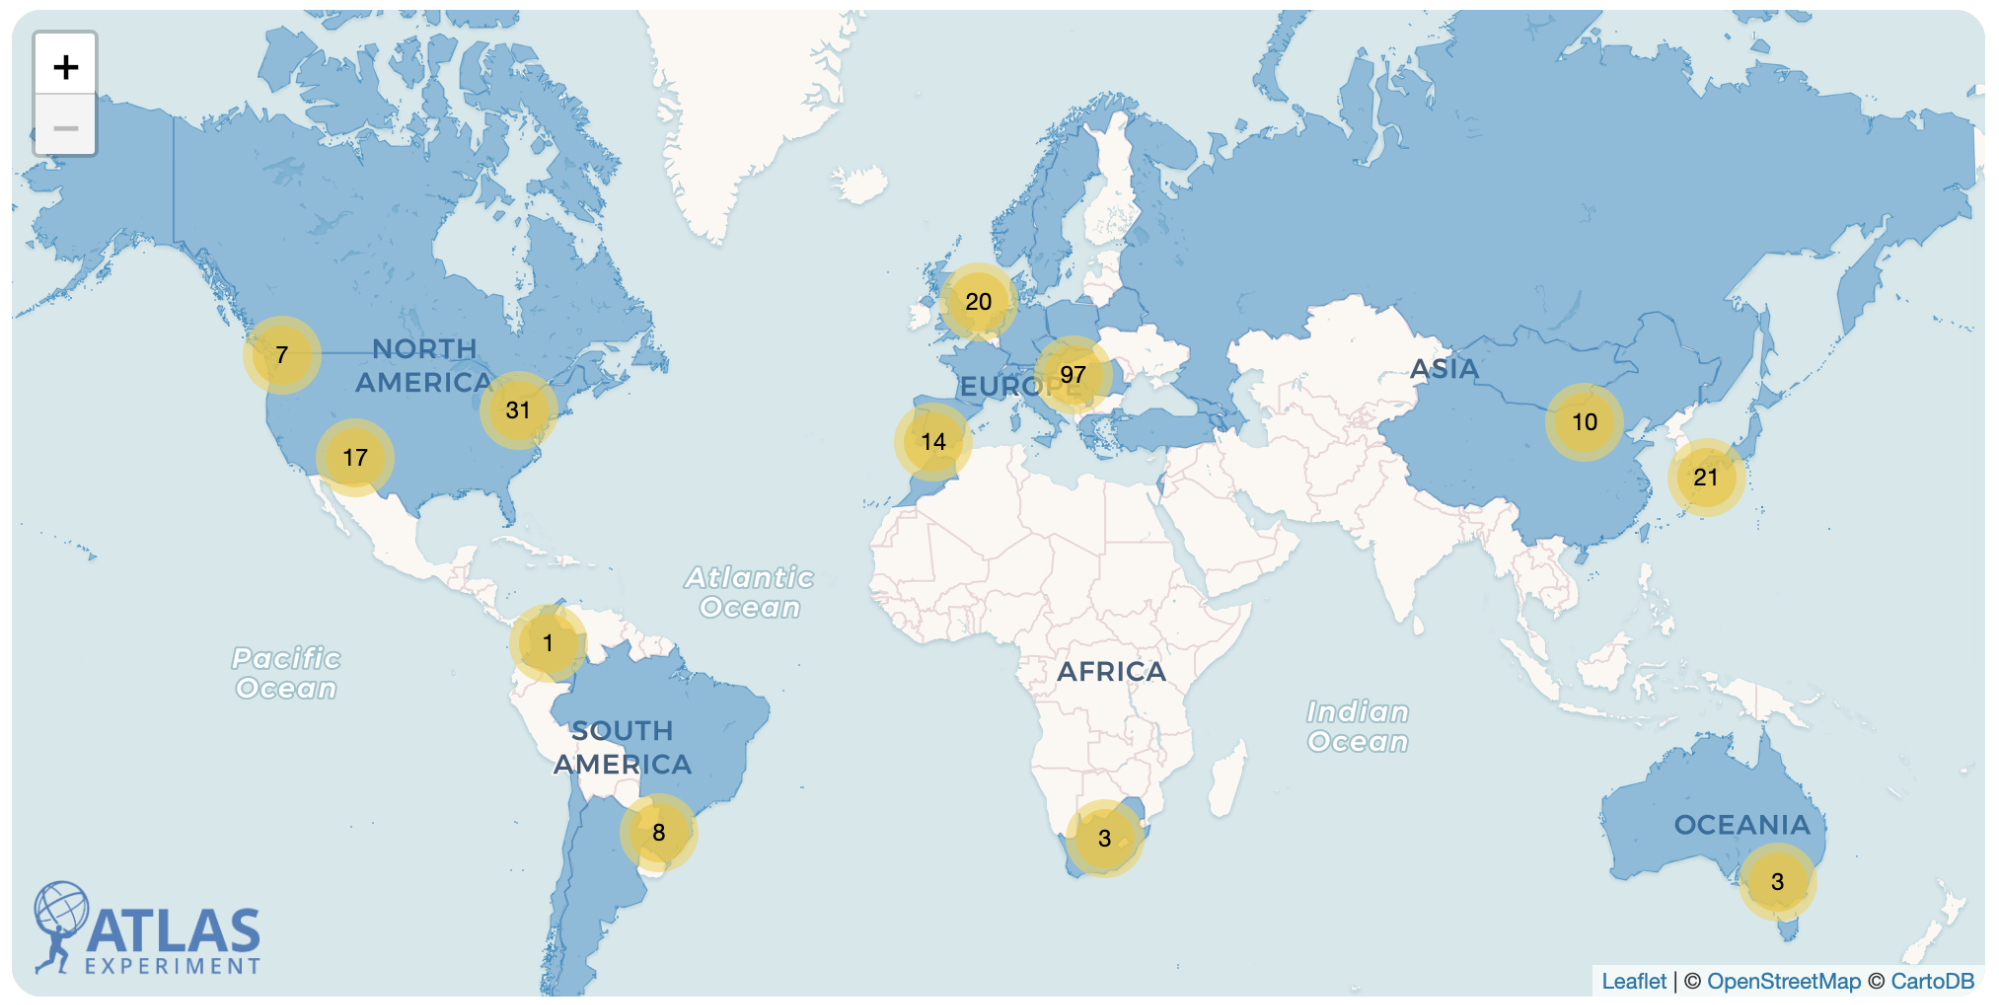
\includegraphics[width=0.9\textwidth]{figures/atlas_map_webpage.png}
  \caption{The ATLAS map webpage.}
  \label{fig:atlas_map_webpage}
\end{figure}
This dynamic webpage filters the results to use only the active institutes. This process is done on ATLAS PO Virtual Machine by a Python script, which makes a request for the API, parses the results, and builds its own JSON file. This file contains all the institutes information (name, country, links, coordinates, etc.) plus the layers to build the map. Once the Python script builds the JSON file, the output is interpreted by the webpage, which takes care of displaying the layers and the markers for the institutes.

\subsection{Data in twiki pages}
\label{sec:Data_in_twiki_pages}

Displaying information into a twiki page requires the use of twiki “\%INCLUDE<path>” function. This function allows to include the content of the <path> file and it will be interpreted by the twiki page. The content could be twiki code or html code. Having html code allows to create more dynamic page. We can use javascript, jQuery and other web development tools to make the content more intuitive to the final user. In this case the page will be loaded on-demand and the data will be displayed on real time thanks to the FENCE framework.

An example of an “include” using an HTML page which retrieves data using the FENCE API and displays it to the user into a twiki page is the public results page (Fig.~\ref{fig:public_twikipage})
\begin{figure}[ht!]
  \centering
  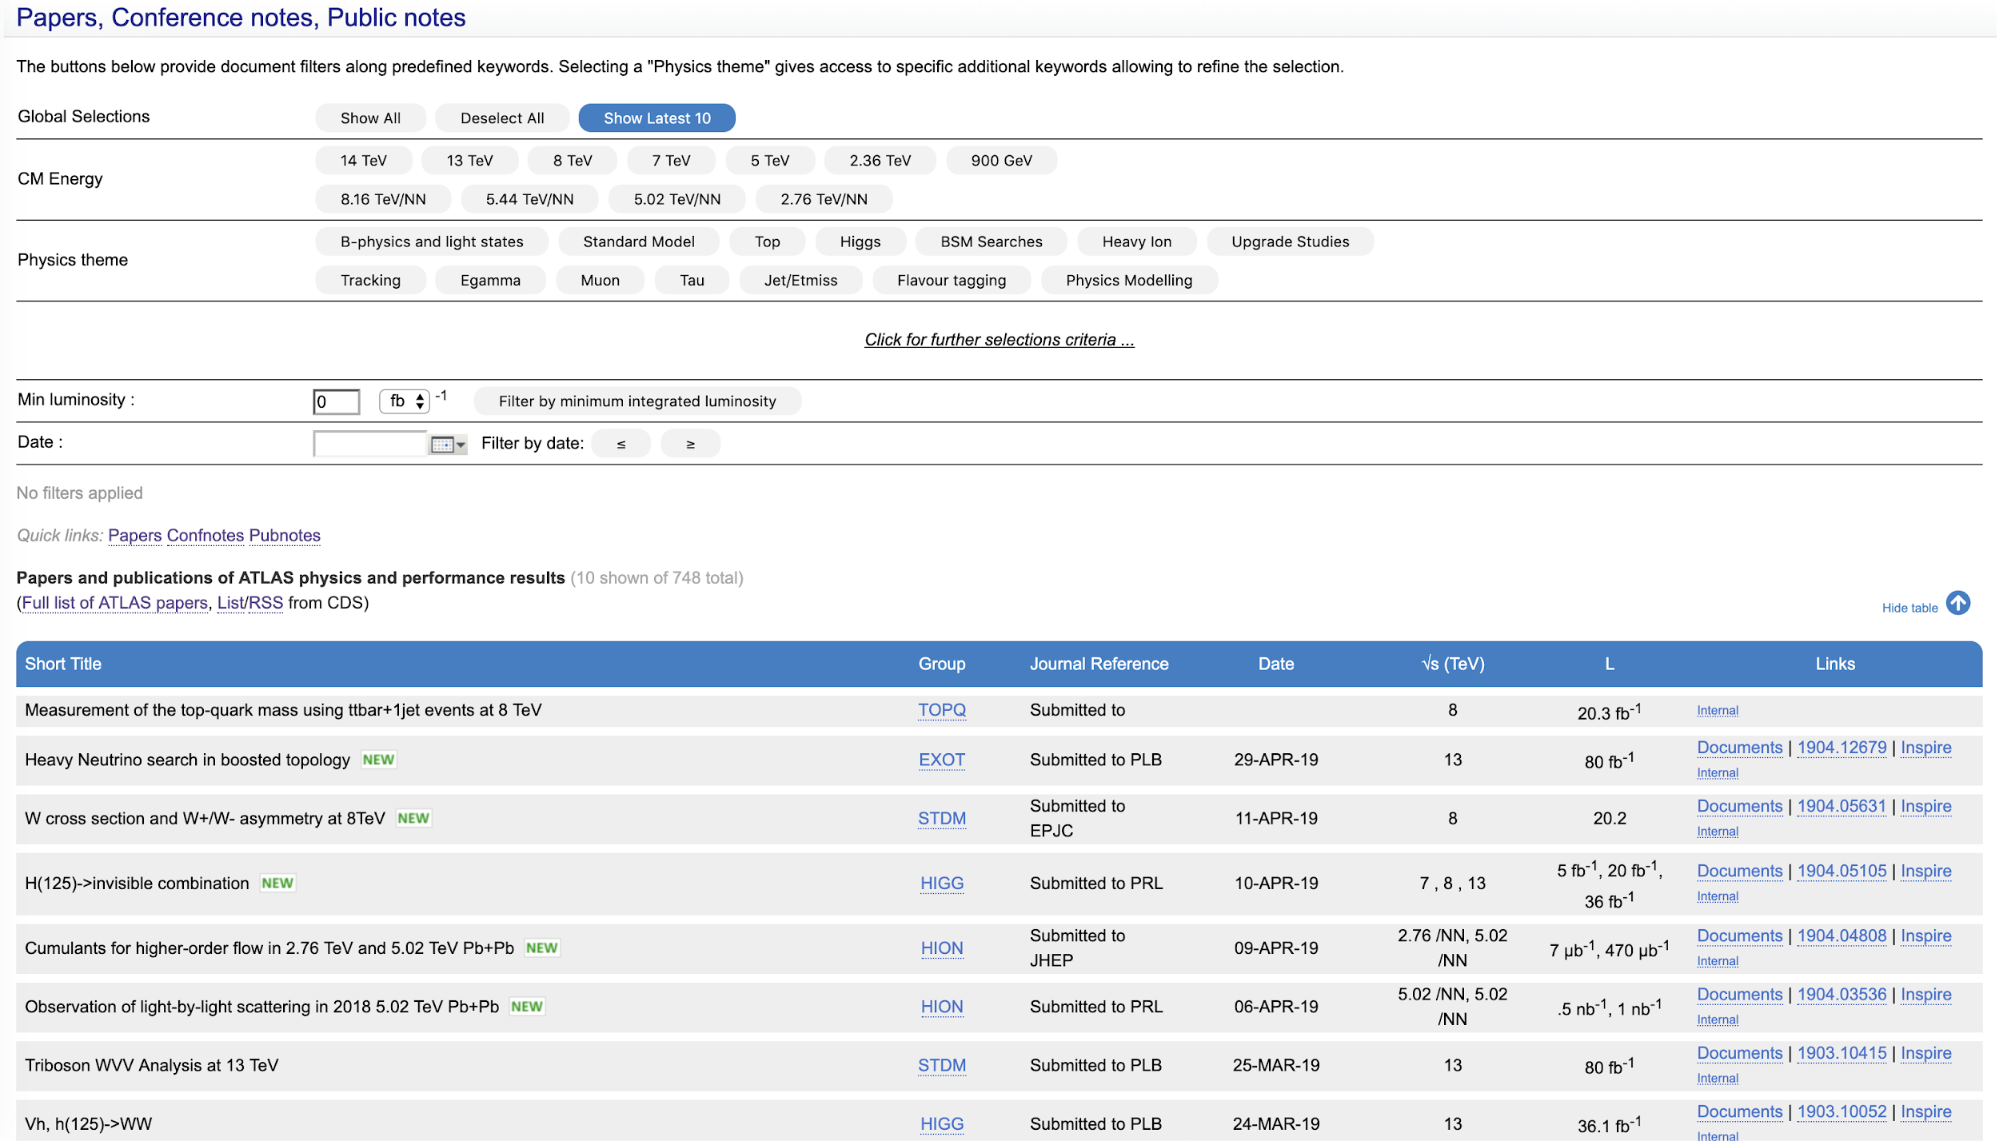
\includegraphics[width=0.9\textwidth]{figures/public_twikipage.png}
  \caption{Public results twiki page.}
  \label{fig:public_twikipage}
\end{figure}

This page shows the full list of Papers, CONF notes or PUB notes stored into ATLAS database and managed by the FENCE framework. It also allows users to filter results using the buttons on the top of the page. This page loads ~1300 records with all the related information. Retrieving all these records at once requires a lot of time. To avoid this, the page initially loads only the first 10 records of each sections and makes the page available for user interaction, then on the background it loads the other records. This solution allows to speed up the loading process and avoids users to wait for the complete data loading.

\subsection{Data on FENCE public pages}
\label{sec:Data_on_FENCE_public_pages}

FENCE allows also to generate public web pages into its own framework instead of using other tools to retrieve and make the information into a human-readable format. This solution is the preferred one since the final data is displayed on call (real time information) and allows the use of all the FENCE’s functionalities and classes that will ease the build and the maintenance of the web page.
